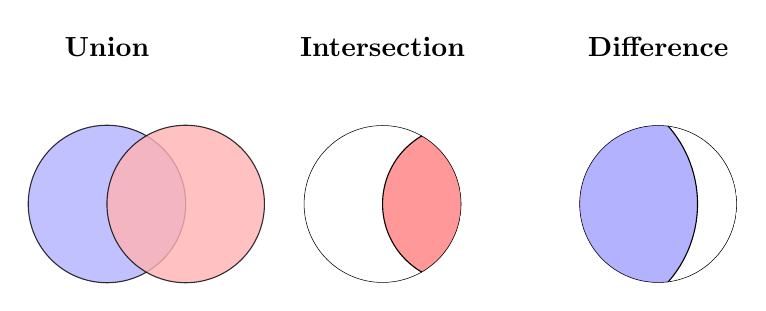
\begin{tikzpicture}
  % Labels
  \node at (-3.5,2) {\textbf{Union}};
  \node at (0,2)     {\textbf{Intersection}};
  \node at (3.5,2)   {\textbf{Difference}};

  % Union
  \begin{scope}[shift={(-3.5,0)}]
    \draw[fill=blue!30,opacity=0.8] (0,0) circle (1);
    \draw[fill=red!30,opacity=0.8] (1,0) circle (1);
  \end{scope}

  % Intersection
  \begin{scope}[shift={(0,0)}]
    \clip (0,0) circle (1);
    \fill[red!40] (1,0) circle (1);
    \draw (0,0) circle (1);
    \draw (1,0) circle (1);
  \end{scope}

  % Difference
  \begin{scope}[shift={(3.5,0)}]
    \clip (0,0) circle (1);
    \fill[blue!30] (-1,0) circle (1.5);
    \draw (0,0) circle (1);
    \draw (-1,0) circle (1.5);
  \end{scope}
\end{tikzpicture}
